


\textbf{Titel}: Laser Refraktion und Reflezion

\textbf{Fuktionsweise} Mit einem Laser wird der Schnee sowohl durchleuchtet für die Refraxion als auch angeleuchtet für die Reflexion. Flüssiges Wasser bildet wegen seiner Oberflächenspannung konkave linsen auf den Prismen des Eis kristalle. Die grösse und damit die Brennweite ändert sich, je nach dem wieviel Volumen Wasser auf den Eiskristallen ist. Die Effekte der Linsen sollten in der Refraxion sichtbar werden. i

In der Reflexion andert sich mit änderndem LWC auch die Oberfläche an der das licht gespiegelt wird.

Der TRL für Refraxion und Reflexion ist bei 2.

\textbf{Beispiele in anderen Sektoren}
Refraxion wird in der Kristalografie angewant.

und Reflexion wird bei einem auflicht mirkoskop immer angeendet.

Die reflexion von wasser an einer Glasscheibe wird genutzt um bei Autos niederschlag auf der windschutztscheibe zu messen.

in beiden Flällen ist hier das TRL 9.

\textbf{Literatur zu Reflexion}
Reflexion von IR
In 20XX hat Herr XX die Reflexion von IR genutzt um den LWC von Schnee zu bestimmen. Die Ergebnisse wurden im Journal XX veröffentilcht.

\textbf{benutzte Mittel für den Versuchsaufbau}
Als Laserquelle wurde ein grüner Bosch Quingo Kreuzlaser genutzt.

Um sowohl die Reflexion als auch die Refraxion gleichzeitig zu sehen, wurde die Schneeprobe auf einen Mikroskopier Objekt träger plaziert.

die Ergebnisse des Lasers wurden jeweils auf weissem Druckpapier dargestellt. Die Refraxion wird auf dem Papier an der Unterseite der Holzplatte dargestellt.

mit dem Fairphone 3 wurde eine Video aufnahme gemacht, wie sich die Ergebinnse des Lasers verändern.

mit einem Kosmetik Spiegel wurde sowohl die reflexion unten als auch die Refraxion oben gleichzeitig in einem Bild dargestellt.

Um alle Teile in fixen relationen zu halten wurde Stativmaterial genutzt.

In Bild \ref{LaserAufbau} ist die Anordnung der Verschieden Teile auf den Stativmaterial zu sehen.

\textbf{Funktionsweise des Versuchsaufbaus}
Der schnee wird in trockenem Zustand bei -10 gard aus dem Gefrieschrank auf den gekühlten Objektträger gelegt. dann wird beobachet wie sich die Ergebnisse ändern wenn der schnee an der Raumtemperatur Luft schmiltzt. Dieser Schmelzvorgang hat rund 5 min gedauert.

der laser scheint durch den Objektievtrager und den schnee durch. dann wird das Lich auf den Papier erneut in die Kamera reflektiert.

die reflexion geschiet zum einen direkt am objektträger, als auch danach im schnee. dieser Aufbau ist suboptimal, denn die konstante reflexion des Objetträgers muss aus dem Laser Ergebniss rausgerechnet werden.

Um Störlicht zu minimieren wurde zuerst eine Einhausung geplant. der durchgeführte verusch hat dann aber einfach in einenm abgedunkelten Raum statt gefunden.

\begin{figure}
    \centering
    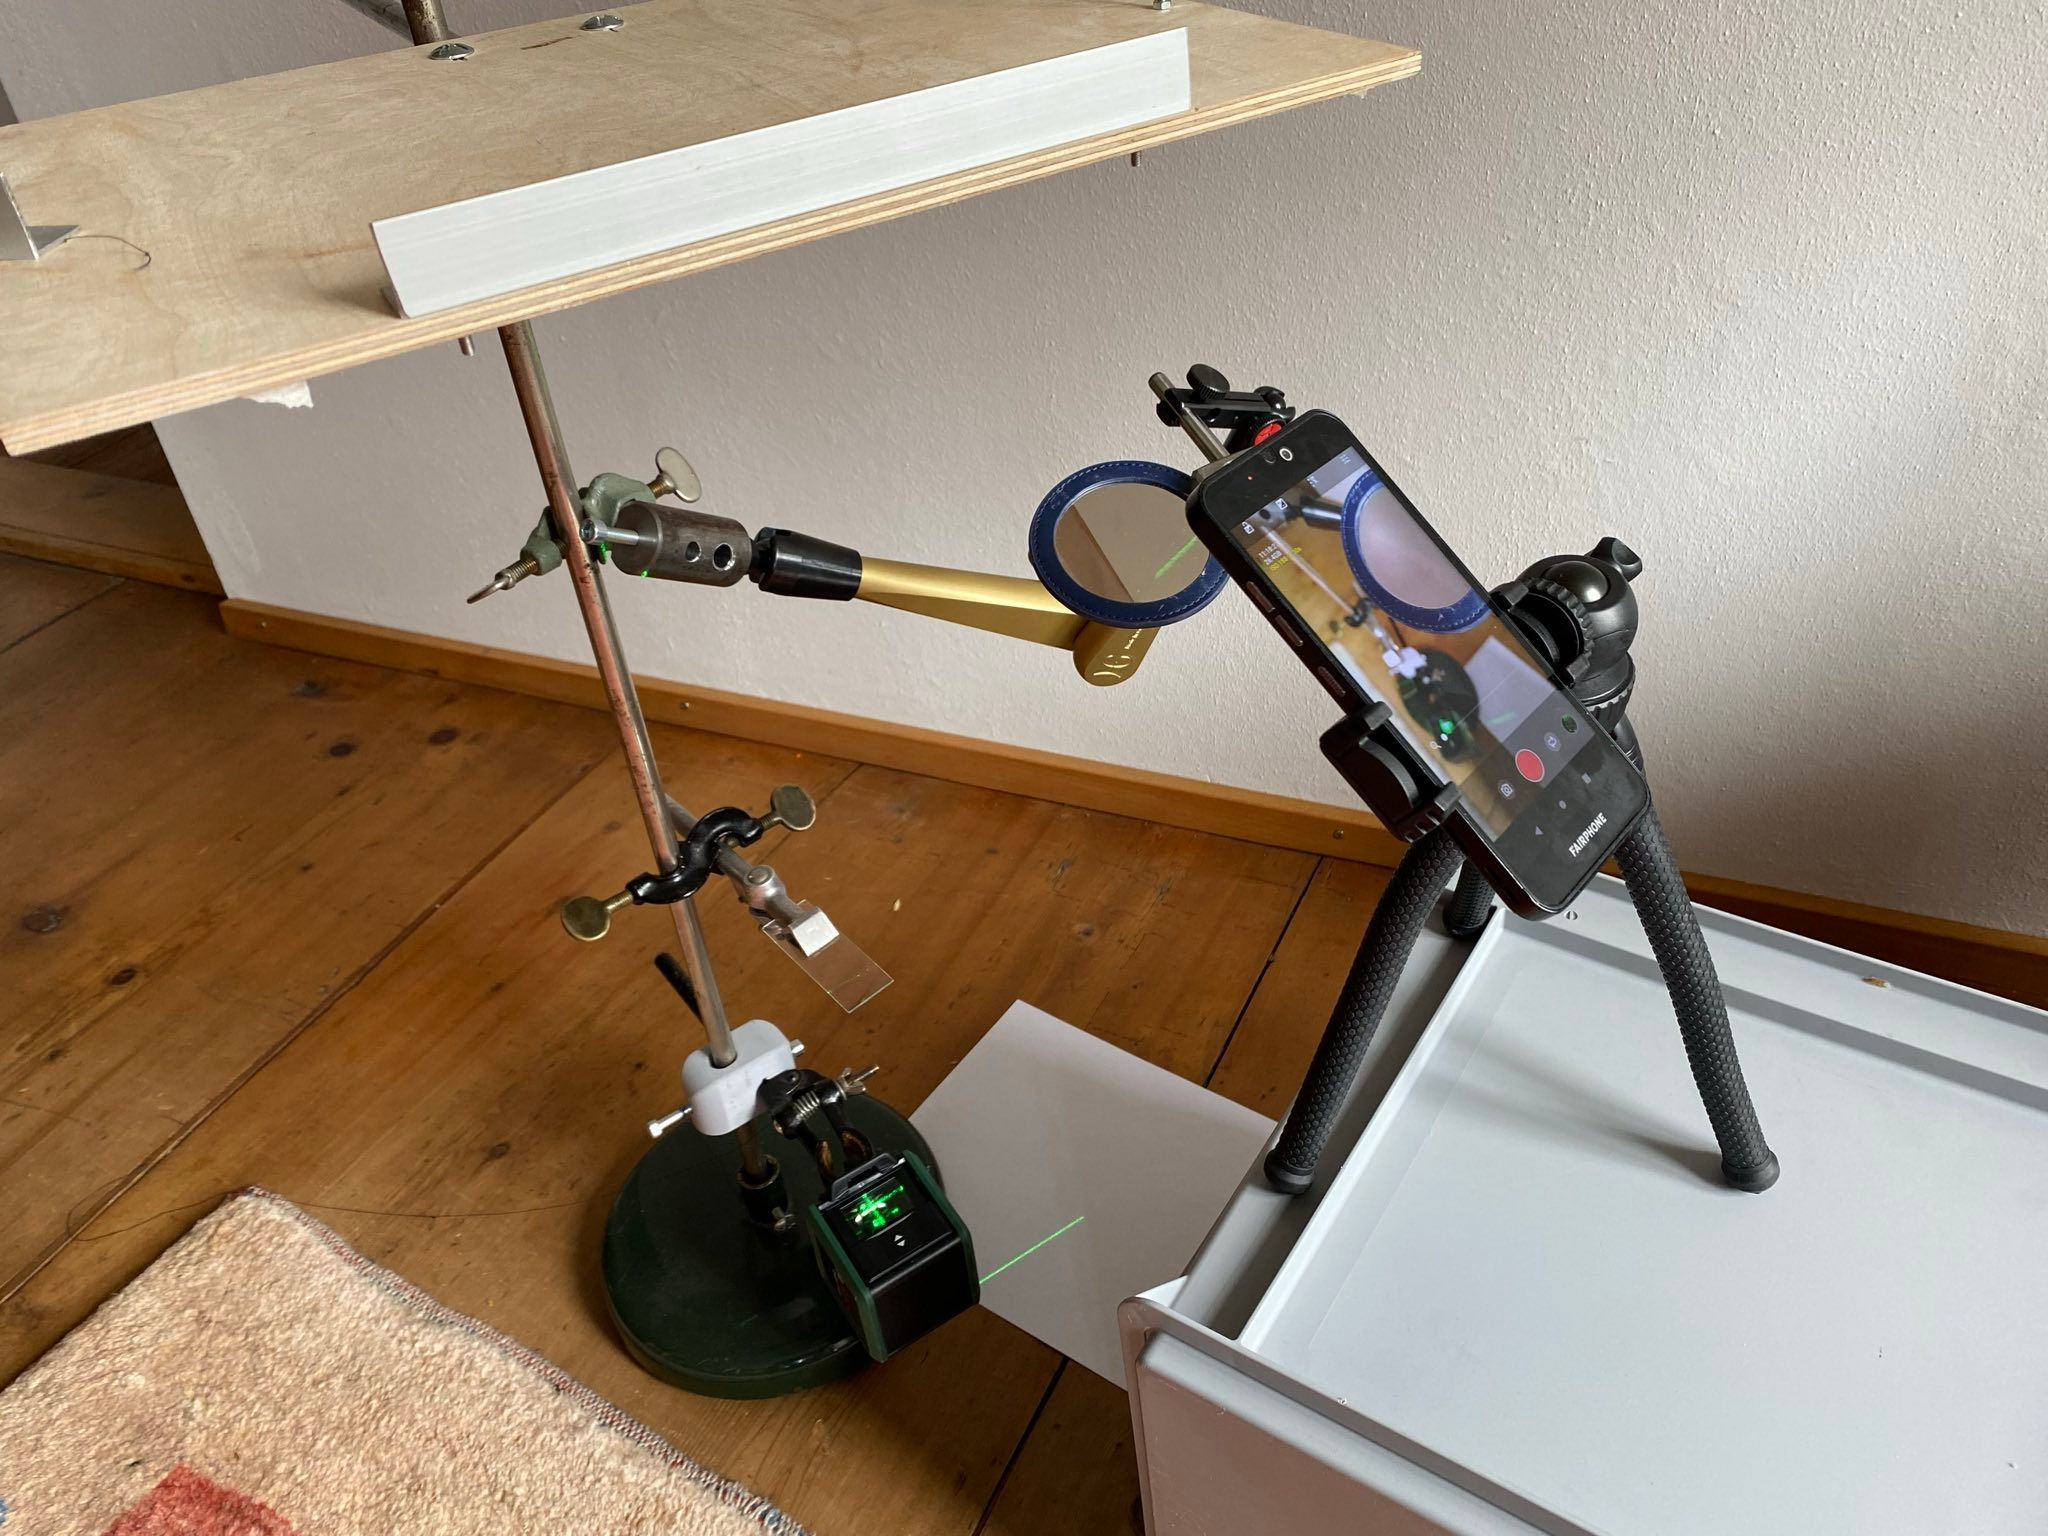
\includegraphics[width=0.8\textwidth]{Bilder/signal-2024-03-10-112013_006.jpeg}
    \caption{Benutzer der Datenbank}
    \label{fig:LaserAufbau}
\end{figure}



\textbf{Messgrössen}
die Anhäufungen von Licht, und die Intesität wird begutachtet.

\textbf{Versuchsergebnisse}

Im bild \ref{LaserBase} ist die Reflexion und refraxion des Objektträges sichtbar. diese konstanten werte müssen von allen Ergebissen subrtahiert werden

\begin{figure}
    \centering
    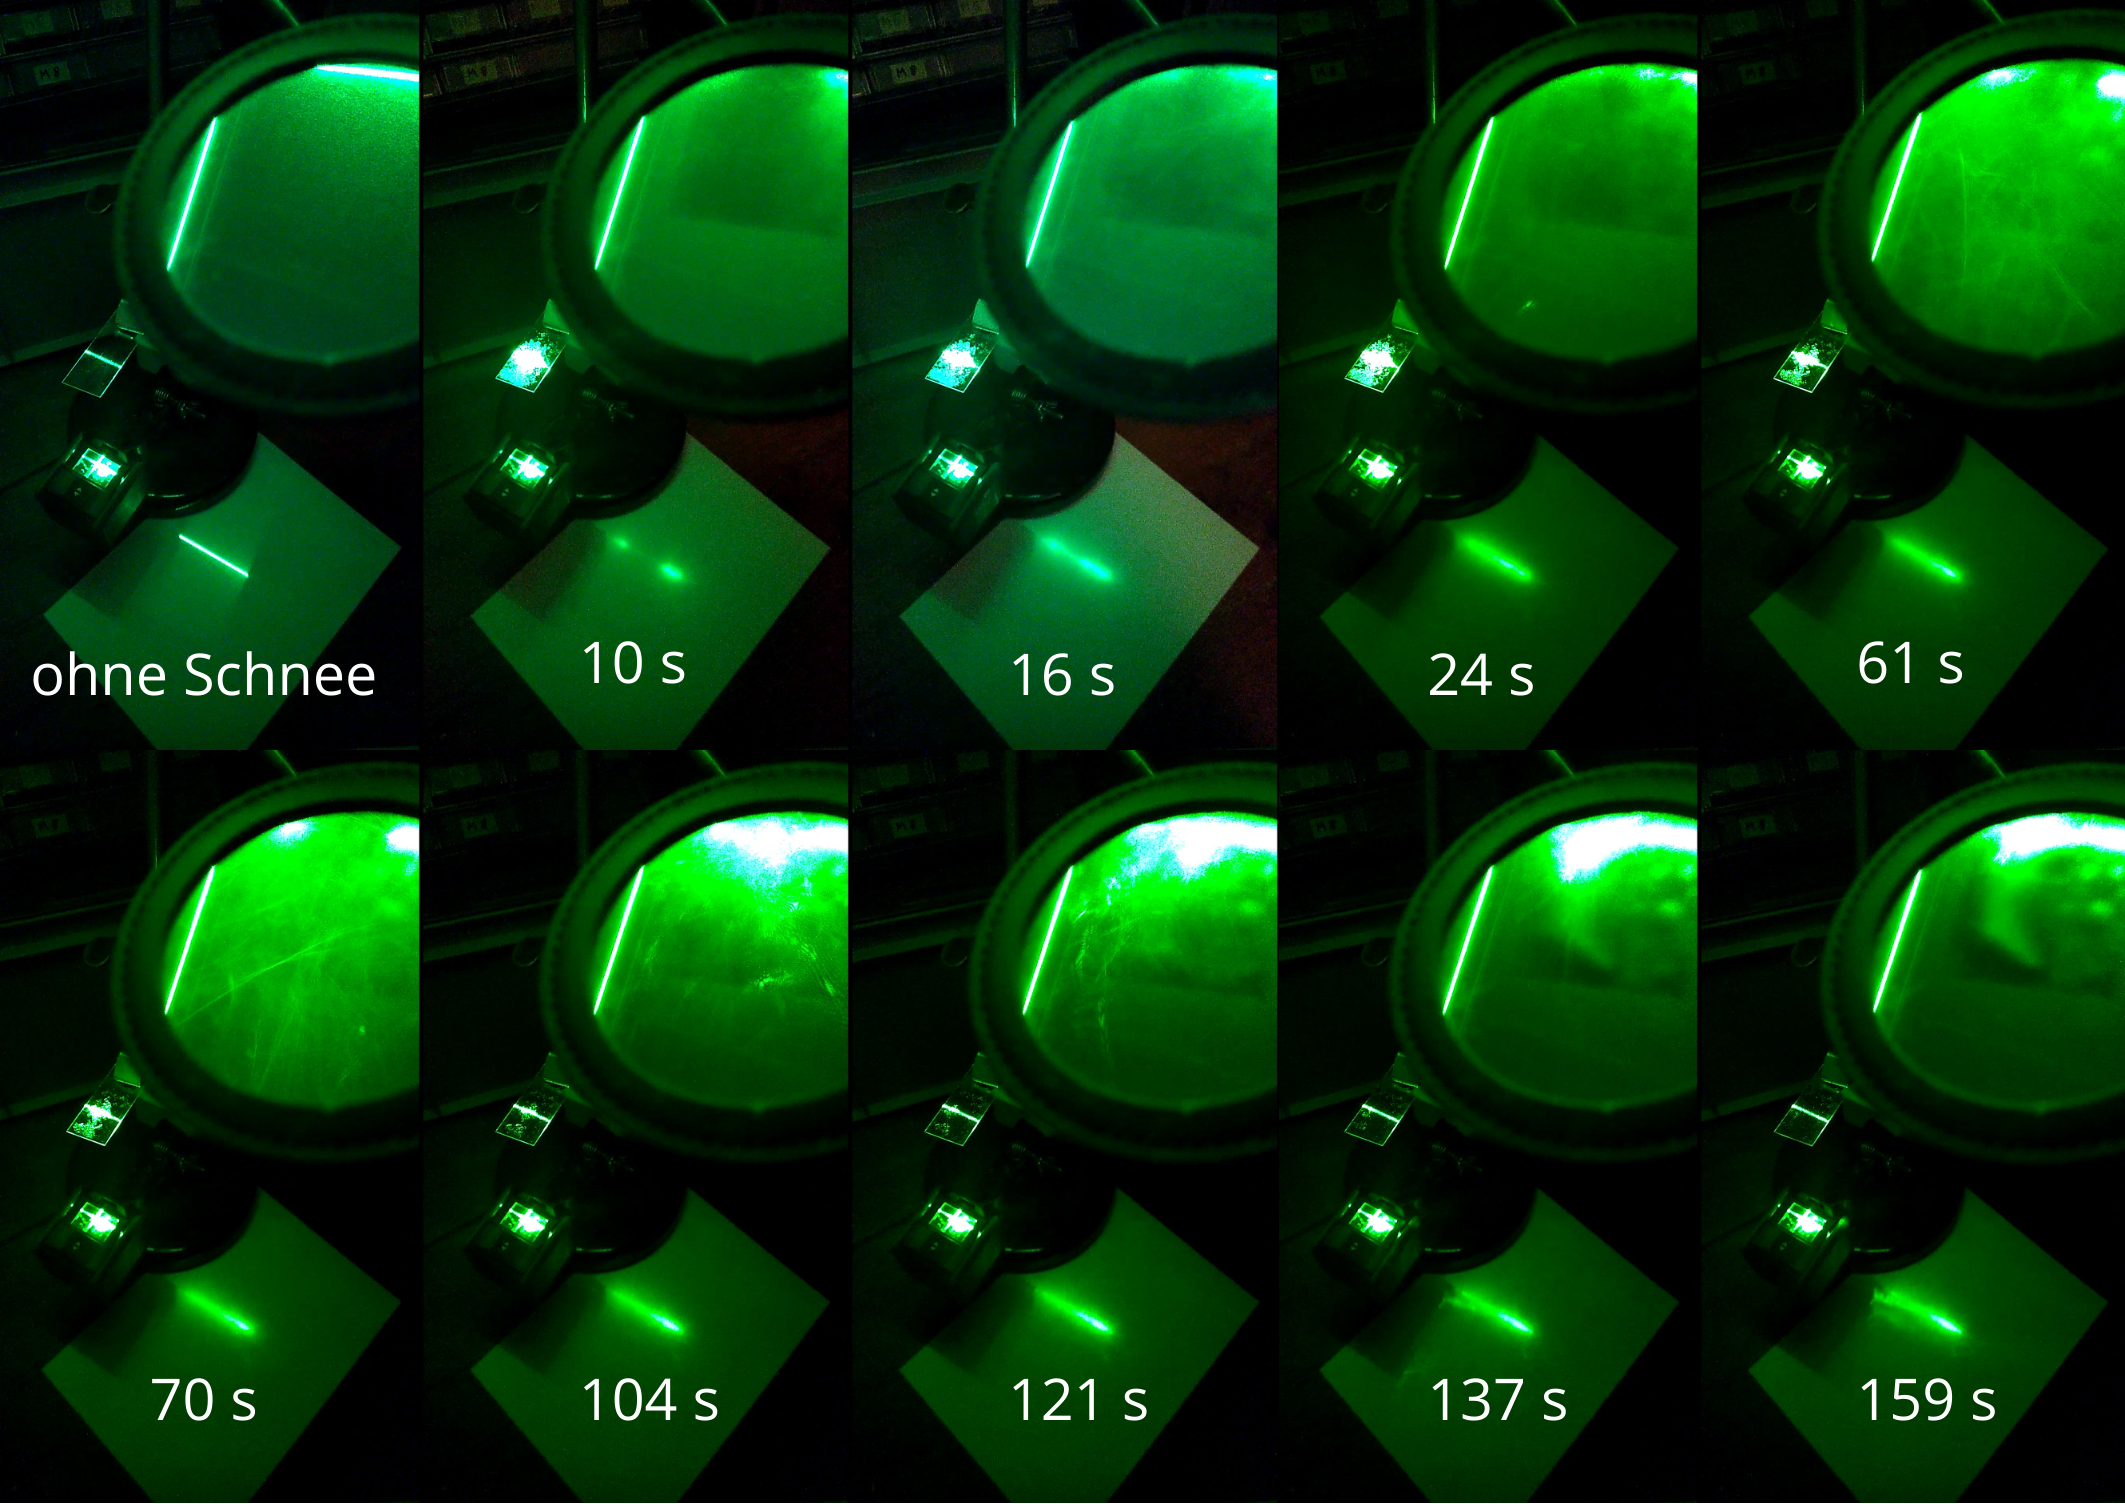
\includegraphics[width=0.8\textwidth]{Bilder/Screenshotfrom2024-04-0413-27-28.png}
    \caption{Benutzer der Datenbank}
    \label{fig:LaserRef}
\end{figure}


\textbf{Aussagekraft der Ergebnisse über den LWC} Die Ergebnisse werden direkt von Wasser beeinflusst. Um den Gewichts LWC zu erhalten, ist aber die geometier der Eiskristalle von extermer Entscheidung. daher ist das Ergebniss nicht direkt mit den LWC überzuführen. Mit der 3D geometire der kristalle wäre ist die Aussagekraft gut.

\textbf{Reflexion zum Versuchsaufbau}
da zwei techniken gleichzeitig gemessen wurden, war der Versuchsaufbau nicht optimal für beide Messgrössen.

Mit den ergebnissen der refraxion bin ich sehr zu frienedn.

\textbf{Verbesserungen des Versuchsaufbaus}
um besser Reflexionsergebnisse zu bekommen keinen Objektrager nutzte, sondern direkt auf schnee.

Für eine statische Messung einer schneeprobe muss die Luft um den schnee herum gekühlt sein. ein Ansatz dafür wird im Vorversuch \ref{TinteVersuchsaufbau} umgestetzt.

Mit dem Laser wird Energie in den Schnee eingebracht. um das schmelzen und damit verfälschen des LWC zu minimiren sollte ein möglichst schwacher Laser eingesetzt werden.

\textbf{weiterverfolgung der physikarischen methoden}
Das Ergebniss der Refraxion zeigt, dass diese Moethode umgesetzt werden könnte. Um vergleichbare werte zu bekommen ist die kristallgeometrie abre von bedeutung. die messung der geometier übersteigt das ausmass der BA. Um eine Messung durchzuführen muss eine sChneeprobe durchleuchtet werden. um das zu erreichen muss der schnee physikalisch aus der schneedecke extrahiert werden. das ist aufwendig. daher wird die Refraxion nicht weiter verfolgt.

das Ergebniss der reflexion ist schwer zu beurteilen. in \ref{} ist die reflexion von EM Wellen bereits untersucht worden. daher wird die Reflexion nicht weiter untersucht.


